\chapter{Empirical Analysis}

\fbox{
    \parbox{\textwidth}
    {
        Chapter Overview
        \begin{itemize}
            \item Applying Bayesian \acp{cnn} for the task of Image Recognition on MNIST, CIFAR-10, CIFAR-100 and STL-10 datasets.
            \item Comparison of results of Bayesian \acp{CNN} with Normal \acp{cnn} architectures on similar datasets.
            \item Regularization effect of Bayesian Network with dropouts.
            \item Distribution of mean and variance in Bayesian \acp{cnn} over time. 
            \item Parameters comparison before and after model pruning. 
        \end{itemize}
    }
}

\pagebreak

\section{Experimentation Methodology} \label{experiments}
For all conducted experiments, we implement the foregoing description of Bayesian \acp{cnn} with variational inference in LeNet-5 \cite{lecun1998gradient} and AlexNet \cite{krizhevsky2012imagenet}. The exact architecture specifications can be found in the Appendix and in our GitHub repository\footnote{\url{https://github.com/kumar-shridhar/PyTorch-BayesianCNN}}.
We train the networks with the MNIST dataset of handwritten digits \cite{lecun1998gradient}, and with the CIFAR-10 and CIFAR-100 datasets \cite{krizhevsky2009learning} since these datasets serve widely as benchmarks for \acp{cnn}' performances. The originally chosen activation functions in all architectures are \textit{ReLU}, but we must introduce another, called \textit{Softplus}, see \eqref{softplus}, because of our method to apply two convolutional or fully-connected operations. As aforementioned, one of these is determining the mean $\mu$, and the other the variance $\alpha \mu^2$. Specifically, we apply the \textit{Softplus} function because we want to ensure that the variance $\alpha \mu^2$ never becomes zero. This would be equivalent to merely calculating the MAP, which can be interpreted as equivalent to a maximum likelihood estimation (MLE), which is further equivalent to utilising single point-estimates, hence frequentist inference. The \textit{Softplus} activation function is a smooth approximation of \textit{ReLU}. Although it is practically not influential, it has the subtle and analytically important advantage that it never becomes zero for $x \rightarrow -\infty$, whereas \textit{ReLU} becomes zero for $x \rightarrow -\infty$.
\\ 
\begin{equation}\label{softplus}
     \text{Softplus}(x) = \frac{1}{\beta} \cdot \log \big ( 1 + \exp(\beta \cdot x) \big )
\end{equation}
\\
where $\beta$ is by default set to $1$.
\newline All experiments are performed with the same hyper-parameters settings as stated in the Appendix.

\section{Case Study 1: Small Datasets (MNIST, CIFAR-10, STL-10)}
\subsection{Datasets}
As aforementioned, we train various architectures on multiple datasets, namely MNIST, CIFAR-10, and CIFAR-100. 
\newline
\subsubsection{MNIST}
The MNIST database \cite{lecun-mnisthandwrittendigit-2010} of handwritten digits, has a training set of 60,000 examples, and a test set of 10,000 examples. It is a subset of a larger set available from NIST. The digits have been size-normalized and centered in a fixed-size image of 28 by 28 pixels. Each image is grayscaled and is labelled with its corresponding class that ranges from zero to nine.

\newline
\subsubsection{CIFAR-10}
The CIFAR-10 are labeled subsets of the 80 million tiny images dataset \cite{Torralba:2008:MTI:1444381.1444403}. The CIFAR-10 dataset has a training dataset of 50,000 colour images in 10 classes, with 5,000 training images per class, each image 32 by 32 pixels large. There are 10000 images for testing. 
\newline
\subsubsection{CIFAR-100}
This dataset is similar to the CIFAR-10, and is a labeled subset of the 80 million tiny images dataset \cite{Torralba:2008:MTI:1444381.1444403}. The dataset has 100 classes containing 600 images each. There are 500 training images and 100 validation images per class. The images are colored with a resolution of 32 by 32 pixels.
\subsection{Results}
First, we evaluate the performance of our proposed method, Bayesian \acp{cnn} with variational inference. Table \ref{tab:results} shows a comparison of validation accuracies (in percentage) for architectures trained by two disparate Bayesian approaches, namely variational inference, i.e. \textit{Bayes by Backprop} and Dropout as proposed by Gal and Ghahramani \cite{gal2015bayesian}, plus frequentist inference for all three datasets. Bayesian \acp{cnn} trained by variational inference achieve validation accuracies comparable to their counter-architectures trained by frequentist inference. On MNIST, validation accuracies of the two disparate Bayesian approaches are comparable, but a Bayesian LeNet-5 with Dropout achieves a considerable higher validation accuracy on CIFAR-10, although we were not able to reproduce these reported results.
\begin{table}[b!]
\tiny
    \centering
    \renewcommand{\arraystretch}{1.5}
    \resizebox{\linewidth}{!}{
    \begin{tabular}{ l  c  c  c  c } 
     \hline
      \empty & MNIST & CIFAR-10 & CIFAR-100  \\ [0.75ex]
     \hline
     Bayesian AlexNet (with VI) & 99 & 73 & 36  \\
     
     Frequentist AlexNet & 99 & 73 & 38  \\
     \hdashline
     Bayesian LeNet-5 (with VI) & 98 & 69 & 31  \\
     
     Frequentist LeNet-5 & 98 & 68 & 33  \\
     \hdashline
     Bayesian LeNet-5 (with Dropout) & 99.5 & 83 & \empty \\ 
     \hline \\
    \end{tabular}} 
    \renewcommand{\arraystretch}{1.5}
    \caption{Comparison of validation accuracies (in percentage) for different architectures with variational inference (VI), frequentist inference and Dropout as a Bayesian approximation as proposed by Gal and Ghahramani \cite{gal2015bayesian} for MNIST, CIFAR-10, and CIFAR-100.}
    \label{tab:results}
\end{table}
\newline In Figure \ref{fig:regularisation}, we show how Bayesian networks incorporate naturally effects of regularization, exemplified on AlexNet. While an AlexNet trained by frequentist inference without any regularization overfits greatly on CIFAR-100, an AlexNet trained by Bayesian inference on CIFAR-100 does not. It performs equivalently to an AlexNet trained by frequentist inference with three layers of Dropout after the first, fourth, and sixth layers in the architecture. In initial epochs, Bayesian \acp{cnn} trained by variational inference start with a low validation accuracy compared to architectures trained by frequentist inference. This must deduce from the initialization of the variational posterior probability distributions $q_{\theta}(w|\mathcal{D})$ as uniform distributions, while initial point-estimates in architectures trained by frequentist inference are randomly drawn from a standard Gaussian distribution. The latter initialization method ensures the initialized weights are neither too small nor too large. In other words, the motivation of the latter initialization is to start with weights such that the activation functions do not let them begin in saturated or dead regions. This is not true in case of uniform distributions and hence, Bayesian \acp{cnn}' starting validation accuracies can be comparably low.
%
\begin{figure}[t!] 
\centering
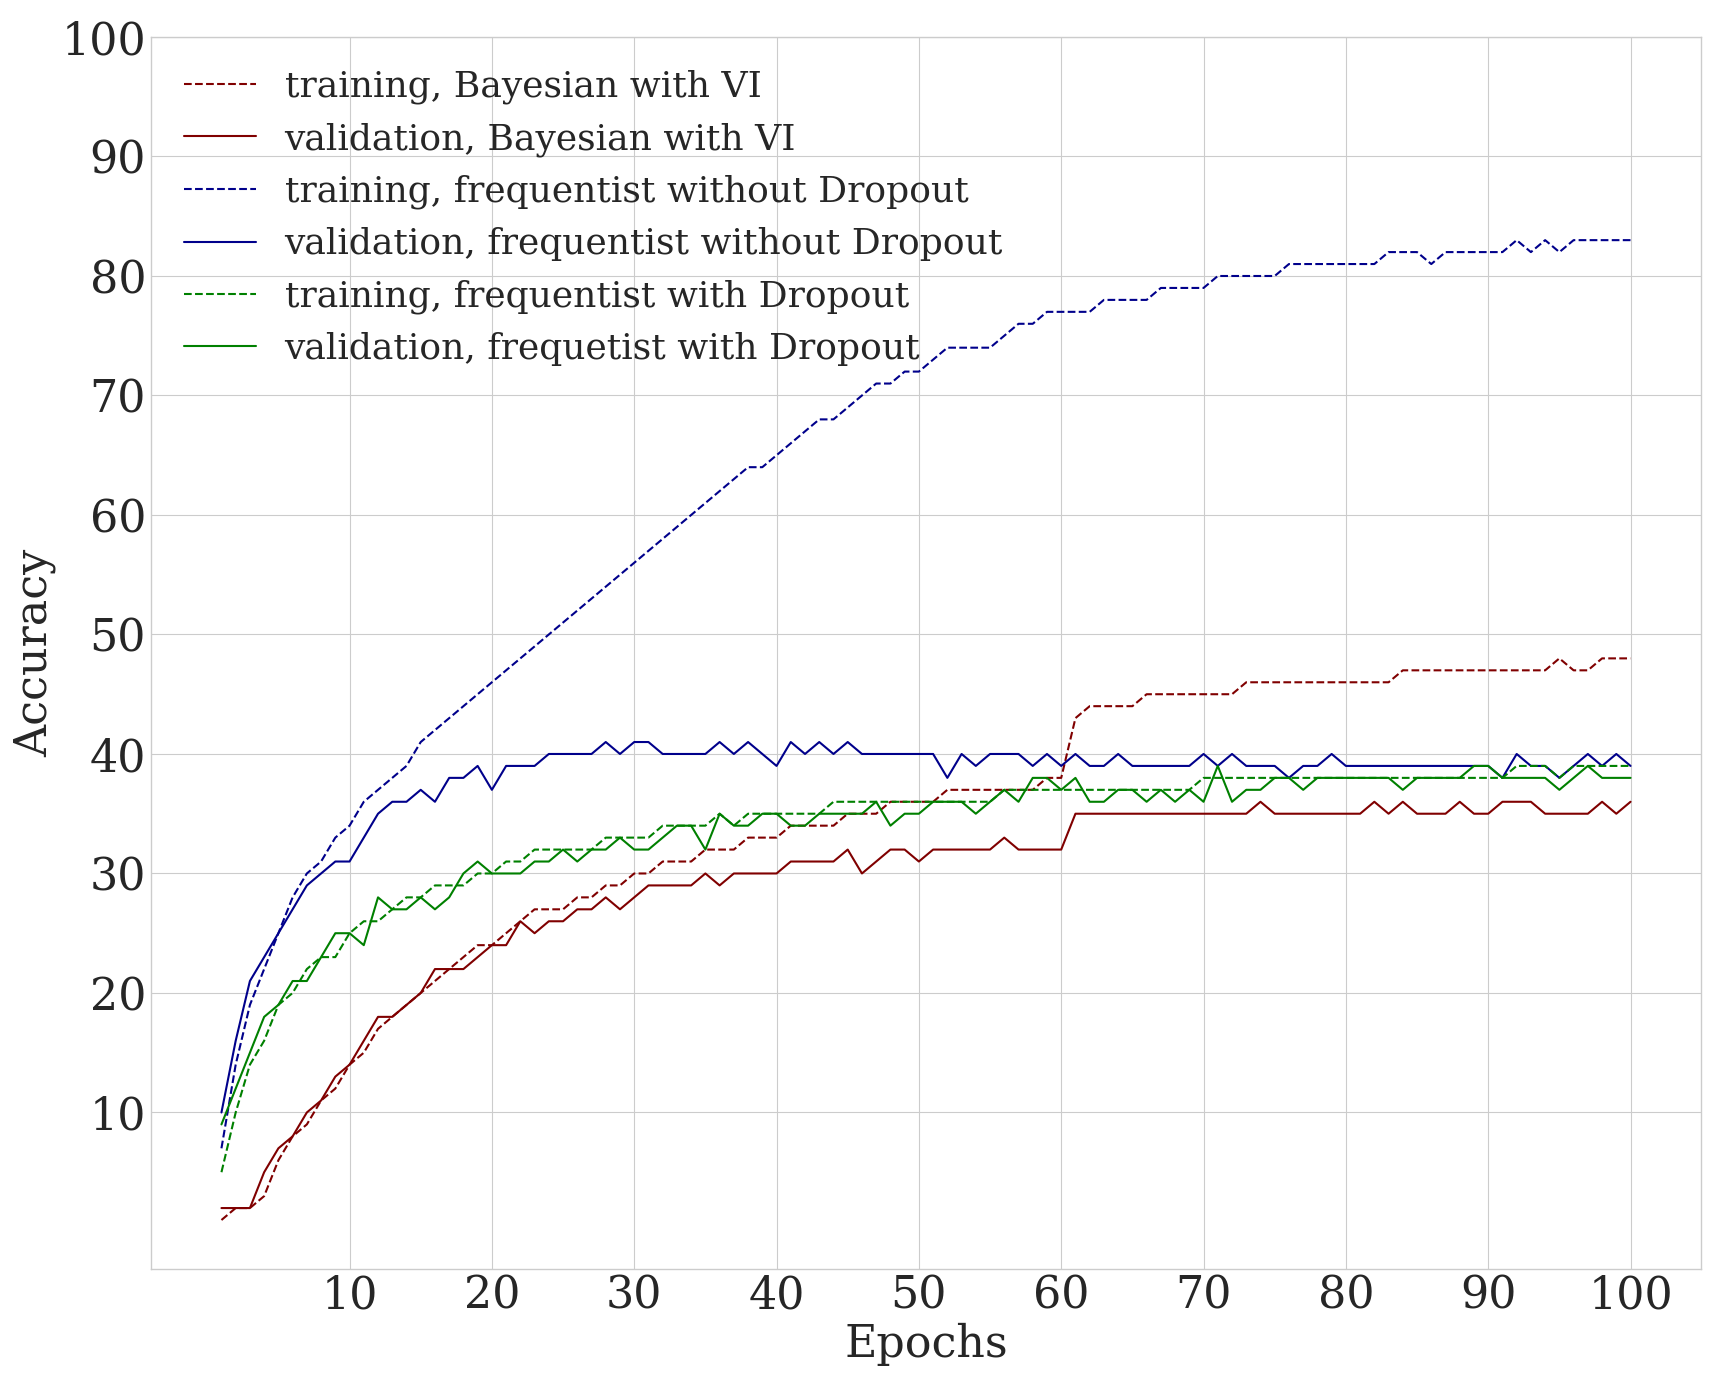
\includegraphics[width=\linewidth]{Chapter5/Figs/results_regularization.png}
\caption{AlexNet trained on CIFAR-100 by Bayesian and frequentist inference. The frequentist AlexNet without Dropout overfits while the Bayesian AlexNet naturally incorporates an effect of regularization, comparable to a frequentist AlexNet with three Dropout layers.}
\label{fig:regularisation}
\end{figure}
%
\newline Figure \ref{fig:std_CNN} displays the convergence of the standard deviation $\sigma$ of the variational posterior probability distribution $q_{\theta}(w|\mathcal{D})$ of a random model parameter over epochs. As aforementioned, all prior probability distributions $p(w)$ are initialized as uniform distributions. The variational posterior probability distributions $q_{\theta}(w|\mathcal{D})$ are approximated as Gaussian distributions which become more confident as more data is processed - observable by the decreasing standard deviation over epochs in Figure \ref{fig:std_CNN}. Although the validation accuracy for MNIST on Bayesian LeNet-5 has already reached 99\%, we can still see a fairly steep decrease in the parameter's standard deviation. In Figure \ref{fig:distribution}, we plot the actual Gaussian variational posterior probability distributions $q_{\theta}(w|\mathcal{D})$ of a random parameter of LeNet-5 trained on CIFAR-10 at some epochs.
%
\begin{figure}[b!] 
\begin{center}
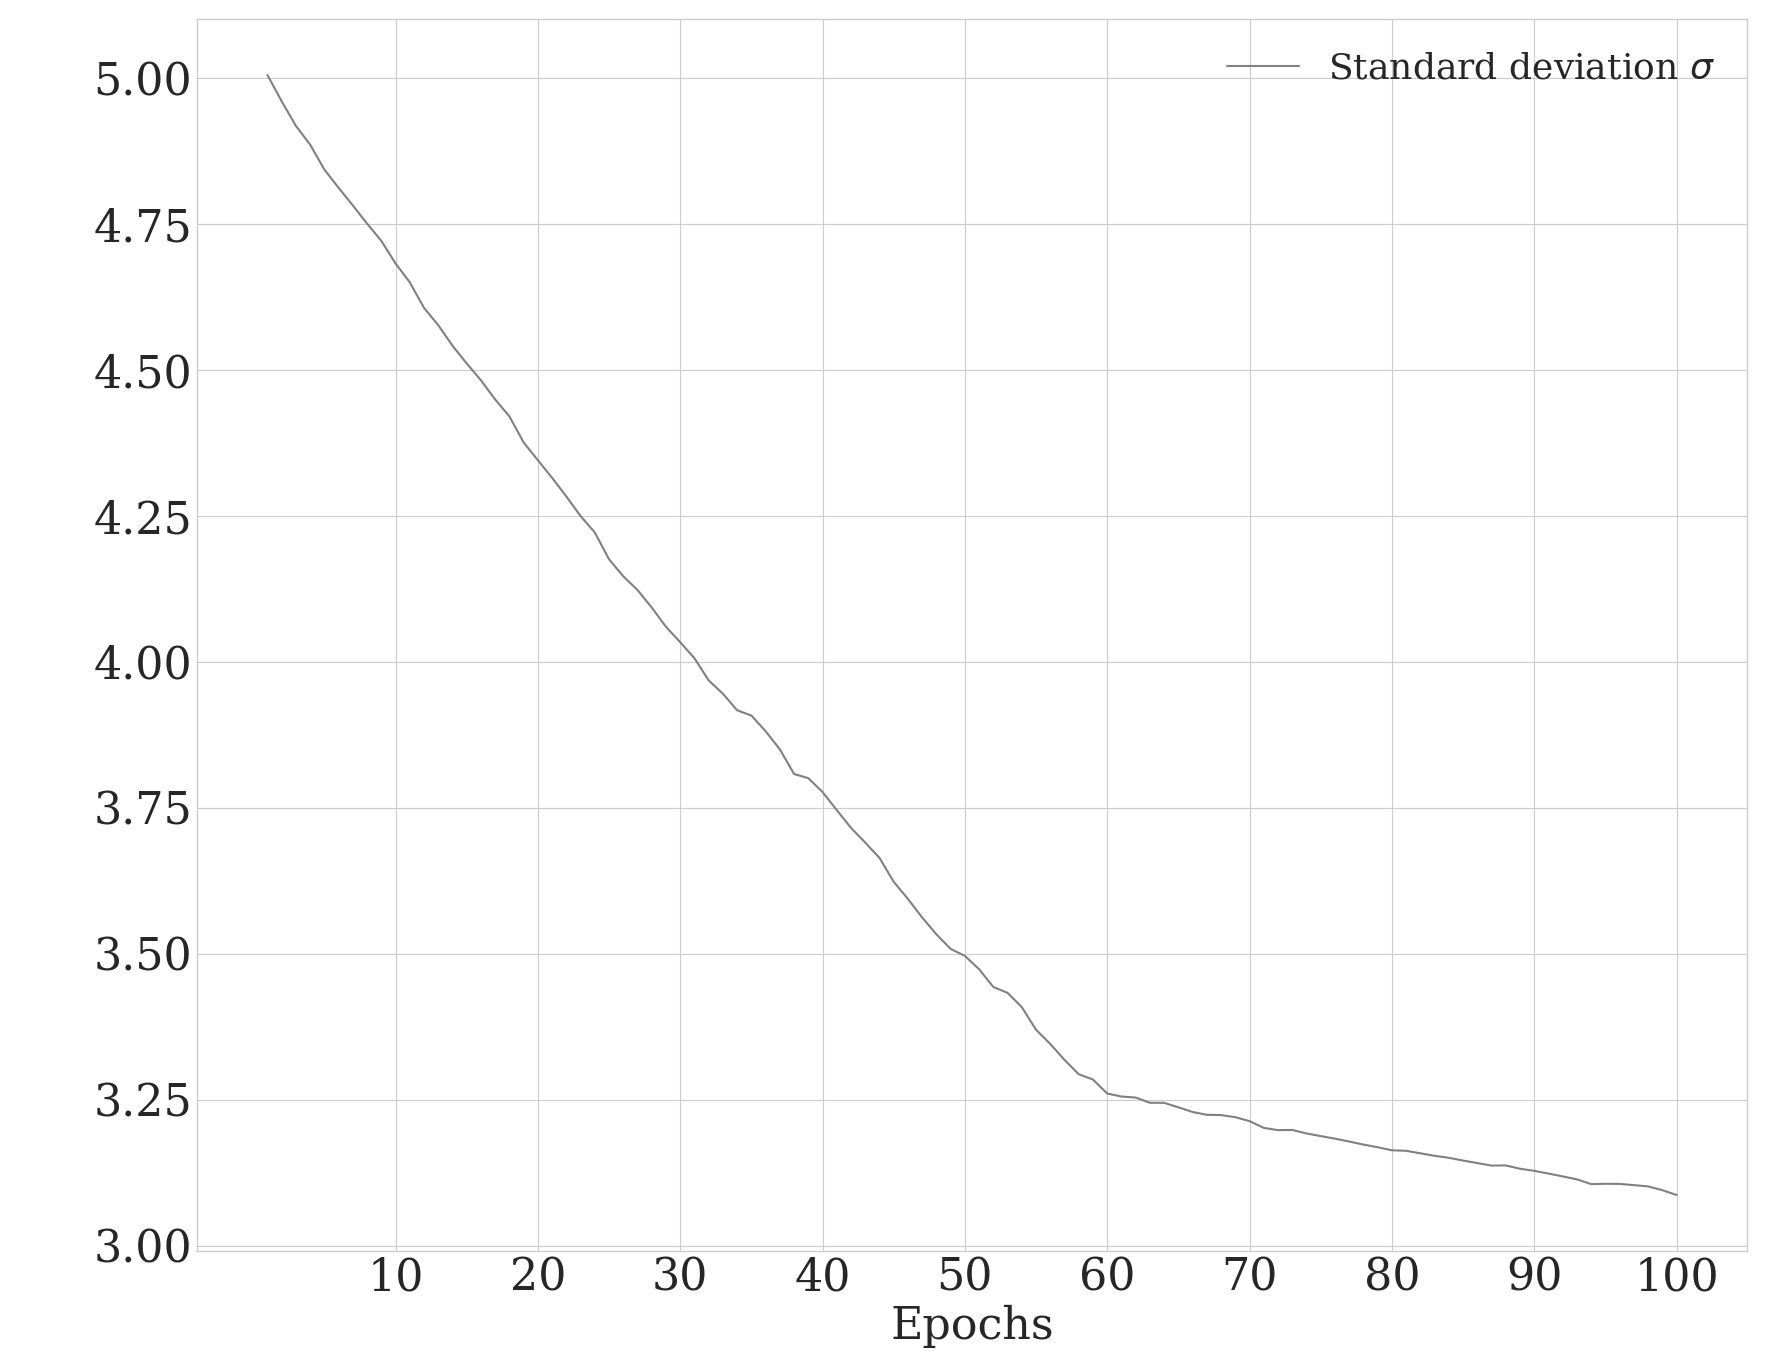
\includegraphics[width=\linewidth]{Chapter5/Figs/std_CNN.png}
\caption{Convergence of the standard deviation of the Gaussian variational posterior probability distribution $q_{\theta}(w|\mathcal{D})$ of a random model parameter at epochs 1, 5, 20, 50, and 100. MNIST is trained on Bayesian LeNet-5.}
\label{fig:std_CNN}
\end{center}
\end{figure} 
%
\begin{figure}[t!] 
\begin{center}
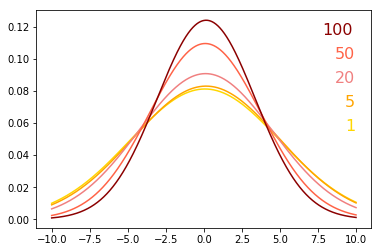
\includegraphics[width=\linewidth]{Chapter5/Figs/distribution.png}
\caption{Convergence of the Gaussian variational posterior probability distribution $q_{\theta}(w|\mathcal{D})$ of a random model parameter at epochs 1, 5, 20, 50, and 100. CIFAR-10 is trained on Bayesian LeNet-5.}
\label{fig:distribution}
\end{center}
\end{figure} 
%
\newline Finally, Table \ref{tab:uncertainty} compares the means of aleatoric and epistemic uncertainties for a Bayesian LeNet-5 with variational inference on MNIST and CIFAR-10. The aleatoric uncertainty of CIFAR-10 is about twenty times as large as that of MNIST. Considering that the aleatoric uncertainty measures the irreducible variability and depends on the predicted values, a larger aleatoric uncertainty for CIFAR-10 can be directly deduced from its lower validation accuracy and may be further due to the smaller number of training examples. The epistemic uncertainty of CIFAR-10 is about fifteen times larger than that of MNIST, which we anticipated, since epistemic uncertainty decreases proportional to validation accuracy. 
\begin{table}[t!]
\tiny
    \centering
    \renewcommand{\arraystretch}{1.5}
    \resizebox{\linewidth}{!}{
    \begin{tabular}{ l  c  c  c  } 
     \hline
      \empty & Aleatoric uncertainty &  Epistemic uncertainty  \\ [0.75ex]
     \hline
     Bayesian LeNet-5 (MNIST) & 0.0096 & 0.0026   \\
     
     Bayesian LeNet-5 (CIFAR-10) & 0.1920 & 0.0404   \\
     \hline \\
    \end{tabular}} 
    \renewcommand{\arraystretch}{1.5}
    \caption{Aleatoric and epistemic uncertainty for Bayesian LeNet-5 calculated for MNIST and CIFAR-10, computed as proposed by Kwon et al. \cite{kwon2018uncertainty}.}
    \label{tab:uncertainty}
\end{table}
%
\section{Case Study 2: Large Dataset (CIFAR-100)}
\subsection{Dataset}
\subsection{Results}

\section{Uncertainity estimation}
\section{Model Pruning}

\ifpdf
    \graphicspath{{Chapter2/Figs/Raster/}{Chapter2/Figs/PDF/}{Chapter2/Figs/}}
\else
    \graphicspath{{Chapter2/Figs/Vector/}{Chapter2/Figs/}}
\fi


